\documentclass[12pt,a4paper]{article}
\usepackage{cite}
%
% with breaklinks=true, links which spanned multiple lines no longer worked...
\usepackage[colorlinks=true,%
            linkcolor=blue,%
            urlcolor=blue,%
            citecolor=blue]{hyperref}
%% modified from http://www.kronto.org/thesis/tips/url-formatting.html
\makeatletter
\def\url@leostyle{%
  \@ifundefined{selectfont}{\def\UrlFont{\sf}}{\def\UrlFont{\small\sffamily}}}
\makeatother
%% Now actually use the newly defined style.
\urlstyle{leo}
%
%% narrower margins, need to be 2cm all round:
\usepackage[margin=2cm]{geometry}  %EPSRC mandated margins
% next two need to add up to 37pt for this to work right, I think:
\setlength{\headheight}{27pt}
\setlength{\headsep}{10pt}
% can't set footskip=0
\setlength{\footskip}{5pt}
%addtolength{\textheight}{5pt}

%% rearrange paragraph indentation and spacing %%
%\setlength{\parindent}{0em}
%\setlength{\parskip}{1.0ex plus 0.5ex minus 0.5ex}
\setlength{\parskip}{0.5ex plus 0.5ex minus 0.5ex}
%\setlength{\parskip}{0ex plus 0.5ex minus 0.1ex}
\parindent 1em % redefine to 1em where paragraph indents are needed
%%% leave off for drafting, then invoke this to help shrink to length!!
%\renewcommand{\baselinestretch}{0.9}  %line spacing squeezed a bit
%%%
%%% table parameters: more space in boxes needed if using lines %%%
%\renewcommand{\arraystretch}{1.3}
%
% for word-wrapped verbatim, use a code listing package:
\usepackage{listings}
\lstset{breaklines=true} 
%%% section headings: smaller font size, less whitespace %%%
\usepackage[small,compact]{titlesec} 
\titleformat{\paragraph}[runin]{\normalsize}{}{0pt}{\bfseries}[ ~]
\titlespacing\paragraph{0pt}{0pt plus 4pt minus 2pt}{0pt plus 2pt minus 2pt}
\titleformat{\section}
{\vspace{0.5ex}%
\titlerule
\vspace{.5ex}%
\large
}
{\thesection.}{0.5ex}{\bfseries\raggedright}
\titlespacing\section{0pt}{0pt plus 4pt minus 2pt}{0pt plus 2pt minus 2pt}
%
%%% change to san serif font %%%
\renewcommand{\sfdefault}{cmss} 
% computer modern sans serif = cmss / phv = helvetica
\renewcommand{\familydefault}{\sfdefault} 
% EPSRC mandated sans serif whole doc (ugh!)
%
%%%%%%%%%%%%%%%%%%%%%%%%%%%%%%%%%%%%%%%%%%%%%
\usepackage[table,dvipsnames]{xcolor} %% can shade in tables
%%% define colours used:
\definecolor{palatine}{rgb}{0.41, 0.16, 0.38} % Durham purple
%
\definecolor{darkgreen}{rgb}{0.05,0.5,0.35} % for WP1
\definecolor{shadegreen}{rgb}{0.75,0.99,0.85}
\definecolor{palegreen}{rgb}{0.85,0.99,0.9} % for workplan timeline
%
\definecolor{darkred}{rgb}{0.5,0.05,0.1} % for WP2
\definecolor{shadered}{rgb}{0.99,0.75,0.85} % for workplan timeline
\definecolor{palered}{rgb}{0.99,0.8,0.9} % for workplan timeline
%
\definecolor{blueviolet}{rgb}{0.05,0.1,0.5} % 
\definecolor{darkblue}{rgb}{0.11,0.11,0.49}
\definecolor{shadeblue}{rgb}{0.8,0.85,0.99}
\definecolor{paleblue}{rgb}{0.85,0.9,0.99} 
%
\definecolor{gray10}{rgb}{0.9,0.9,0.9} % for workplan
\definecolor{gray30}{rgb}{0.7,0.7,0.7} % for workplan
\definecolor{gray50}{rgb}{0.5,0.5,0.5} % for workplan
\definecolor{gray70}{rgb}{0.3,0.3,0.3} % for workplan
%
%% tikz needed for workplan, if not for figures:
\usepackage{tikz}
\usetikzlibrary{shapes,arrows,tikzmark}
\tikzstyle{every loop}=[]
\usepackage{graphicx} %% to include figures
\usepackage{xspace}
%
%%% all the publications listing stuff is in here:
%\usepackage{xr} % for crossrefs if used in bib
%\usepackage[square,numbers,sort&compress]{natbib}
%\bibliographystyle{unsrtnat}
\usepackage{multibib}
%\def\bibsection{\subsection*{\refname}} 
\newcites{pub}{\null\\[-1.3em]}%  \citepub, \nocitepub, ...
\bibliographystylepub{abbrev_unsrt}
\bibliographystyle{abbrev_unsrt}
%\usepackage{doi} % show doi as links
%
\usepackage{paralist} % compact lists
%\usepackage[nodayofweek]{datetime}
%
\newcommand{\inlinebullet}{{\footnotesize\textbullet\ }}
%%%for comments while drafting:
\newcommand{\redit}[1]{\textcolor[named]{Maroon}{\textit{$\bigstar$ #1}}}
\newcommand{\VK}[1]{\textcolor{darkgreen}{VK: #1}}
%%% set up your own, edit to suit:
%\newcommand{\AB}[1]{\textcolor{darkblue}{AB: #1}}
%\newcommand{\HK}[1]{\textcolor{palatine}{HK: #1}}
\newcommand{\NC}[1]{\textcolor{Sepia}{NC: #1}}
\newcommand{\RA}[1]{\textcolor{blue}{RA: #1}}
%%% used for response to referees:
%

\newcommand{\hpc}{High Performance Computing (HPC)\renewcommand{\hpc}{HPC\xspace}\xspace}
\newcommand{\pue}{Power Utilisation Efficiency (PUE)\renewcommand{\pue}{PUE\xspace}\xspace}
\newcommand{\repq}[1]{\textcolor{darkblue}{\textit{#1}}} % repq = referee report quote
\newcommand{\callq}[1]{\textcolor{darkgreen}{#1}}         % callq = Call quote
\newcommand{\redq}[1]{\textcolor{Maroon}{#1}}  % redq = dark red text quote

%%% set up project name and abbreviation here:
\newcommand{\projname}{\textcolor{darkblue}{ICHS}}
\newcommand{\projtitle}{\textbf{\textcolor{darkblue}{\large $\bigstar$ Immersion Cooling and Heat Storage technologies for HPC -- ICHS  $\bigstar$}}}
%%% color-code the work packages throughout:
\newcommand{\WPI}{\textcolor{darkgreen}{WP1}}
\newcommand{\WPII}{\textcolor{darkred}{WP2}}
\newcommand{\WPIII}{\textcolor{darkblue}{WP3}}
%\newcommand{\WPIIIN}{\textcolor{darkblue}{WP3--N}}
\newcommand{\WPIV}{\textcolor{Maroon}{WP4}}
%%% WP5 is black/grey, don't need command
% Above used in Gantt chart, remove when updated...
%
%%% This gives a fairly robust textwidth shaded box:
\newsavebox{\minibox}
\newlength{\minilength}
\newenvironment{framedminipage}[1][\linewidth]{%
  \setlength{\minilength}{#1}
  \addtolength{\minilength}{-2\fboxsep}
  \addtolength{\minilength}{-2\fboxrule}
  \begin{lrbox}{\minibox}\begin{minipage}{\minilength}\raggedright}%
  {\end{minipage}\end{lrbox}\fcolorbox{gray50}{paleblue}{\usebox{\minibox}}}
%
%%% for maths and symbols: %%%
\RequirePackage{amsmath}
\RequirePackage{mathtools} % fixes broken stuff in amsmath
\usepackage{amsfonts}
\usepackage{amssymb}
\usepackage{amsbsy}
%
\usepackage{pgfgantt} % to draw Gantt chart
%
% reduce space wasted by allowing text and big figures in a column
\renewcommand\floatpagefraction{.9}
\renewcommand\dblfloatpagefraction{.9} % for two column documents
\renewcommand\topfraction{.9}
\renewcommand\dbltopfraction{.9} % for two column documents
\renewcommand\bottomfraction{.9}
\renewcommand\textfraction{.1}   
\setcounter{totalnumber}{50}
\setcounter{topnumber}{50}
\setcounter{bottomnumber}{50}

%*********** CHANGE THIS TO SUIT **************************%
\usepackage{fancyhdr}
\pagestyle{fancy}
\fancyhf{}
\fancyhf[LH]{{\tiny \today}}
%\fancyhf[CH]{\textcolor{darkblue}{HACQS}} %{}
\fancyhf[RH]{\thepage}
\renewcommand{\headrulewidth}{0pt}
\renewcommand{\footrulewidth}{0pt}
%
%%% shortcuts: (needed if include tikz ART diagrams)
\def\M{{\cal M}}
\def\C{{\cal C}}
\newcommand{\ket}[1]{\ensuremath{\left|#1\right\rangle}}
\newcommand{\bra}[1]{\ensuremath{\left\langle #1\right|}}
\newcommand{\p}{\mathbf{p}}
\newcommand{\s}{\mathbf{s}}
\newcommand{\RT}{\mathcal{R_T}}
\newcommand{\IRT}{\mathcal{\widetilde{R}_T}}
\newcommand{\theory}{\mathcal{T}}
\newcommand{\see}{C}
%
\begin{document}

\title{GEMS Toolbox manual}
\author{}
\date{10th June 2025}

\maketitle

\tableofcontents

\section{Summary}
This document describes the procedure for setting up a model for mine water heating using the GEMS Toolbox. The procedure makes use of the software tools ArcGIS Pro (commercial software tool), python, gmsh, and Paraview (free software tools).

\section{Contact points}
\begin{tabular}{l l}
    Jeroen van-Hunen: &  jeroen.van-hunen@durham.ac.uk\\
    Julien Mouli-Castillo: & julien.mouli-castillo@glasgow.ac.uk\\
    Yuxiao Wang:& yuxiao.wang@ifg.uni-kiel.de\\
    Steve Shi: & difu.shi@durham.ac.uk
\end{tabular}

\section{Required software tools}
\subsection{ArcGIS Pro or QGIS}
Mine plan digitisation is done using GIS software. At the moment, tools are available for ArcGIS Pro or QGIS.
\subsubsection{ArcGIS Pro}
For staff/students of Durham University, ArcGIS Pro is available through \url{https://appsanywhere.durham.ac.uk/login}, either in one of the computer rooms on the university campus, or on your own computer. Type your CIS username and password, and log in. An 'Open Appsanywhere' pop-up window might appear, which you should agree to. If you are running Appsanywhere for the first time, you may be guided to install it first on your machine. In the search box, search for the latest version of {\tt ArcGIS Pro} (version 3.0 at the time of writing), and click on {\tt Launch Remote}. A 'Parallels Client' remote window will open, which contains ArcGIS Pro.

ArcGIS Pro can also be directly downloaded, and, after creating an account as explained \href{https://durhamuni.maps.arcgis.com/home/index.html}{here}, can be run on your own computer, but only if your computer runs a MS Windows operating system.

\subsubsection{QGIS}
To install the latest stable version, the user is referred to \href{https://docs.qgis.org/3.34/en/docs/user_manual}{the QGIS website}, Section 5.1.

\subsection{Python}
This code requires Python 3, with Python 3.12 or 3.13 being recommended. 

You can set up your environment using either Python's built-in venv module or Conda. For Python installation, visit the official Python website at \url{https://python.org/downloads}. 

If you prefer Conda, you can download and install it from \url{https://docs.conda.io/projects/conda/en/latest/user-guide/install/}. The required package list is located in the directory \texttt{config/GEMS.base.yml}. Instructions for package installation will be provided in a later section. 

To check if the installation was done correctly, do the following:
\begin{itemize}
    \item Open a terminal 
    \item Type: \\
    {\tt which python} (MacOS or Linux)\\
    {\tt where python} (Windows)
\end{itemize}
This should provide you with a full path for the Python executable. 

% \subsection{Gmsh}
% The code for the GEMS Toolbox makes use of a meshing software {\tt Gmsh}, which can be downloaded at \url{https://gmsh.info/#Download}. Make a note of where {\tt Gmsh} is installed, as you will need that information when running the GEMS Toolbox later.

\subsection{Paraview}
The visualisation software tool Paraview can be downloaded from \url{https://www.paraview.org/download/}. The Mac OS versions are all fairly stable, but the MS Windows versions not so much. If the latest version is not working properly, try installing an earlier version. 

\section{Installing and running the GEMSToolbox software}
The GEMSToolbox is designed to import a custom digitised map and test the feasibility of this mine system for mine water geothermal energy purposes. This is all described further down in this manual. This section describes how to install the GEMSToolbox software and test that it runs normally on your computer.


\subsection{Installation of GEMSToolbox}
\begin{enumerate}
    \item Downloading GEMSToolbox
    You should have received a {\tt.zip} file of the code. Please contact jeroen.van-hunen@durham.ac.uk if this is not the case. Unzip the GEMSToolbox zip file into a suitable folder on your computer. We'll call this folder {\tt <homeGEMSTb>} from now on.

    \item Install GEMSToolbox Python environment
    \begin{itemize}
        \item By conda:
            \begin{itemize}
                \item Navigate to the GEMS directory. Then run:
                \begin{itemize}
                    \item \texttt{conda env create -f config/GEMS.base.yml}
                \end{itemize}
                \item Activate GEMS enviroment:
                \begin{itemize}
                    \item \texttt{conda activate GEMS}
                \end{itemize}
            \end{itemize}
        \item By python venv:
            \begin{itemize}
            
            %     \item Install python and pip (if you already done this step, you can ignore this section)
            %     \begin{itemize}
            %         \item Python installation can be found at \url{https://www.python.org/}. After installation, open your terminal and run \textbf{'python'} to verify whether the installation is successful.
            %         \item Pip installation can be found at \url{https://pip.pypa.io/en/stable/installation/}. After installation, open your terminal and run \textbf{'pip -V'} to verify whether the installation is successful. 
            %         \item Create a virtualenv environment.
            %         \begin{itemize}
            %             \item Open a Terminal or Command Prompt: Navigate to the directory where you want to create your virtual environment.
            %             \item Use the venv Module: Enter the command \textbf{'python3 -m venv myenv'}, replacing \textbf{'myenv'} with the name you want to give to your virtual environment:
            %             \item Activate the Virtual Environment:
            %             On Windows, run \textbf{ 'myenv$\backslash$Scripts$\backslash$activate'}. 
            %             On macOS and Linux, run \textbf{'source myenv/bin/activate'}.
            %         \end{itemize}
            %     \end{itemize}
            
            \item In terminal or Windows CMD, to create GEMS venv, run:
                \begin{itemize}
                    \item {\texttt{python -m venv GEMS }}
                \end{itemize}
            \item Activate GEMS venv:
                \begin{itemize}
                    \item On Windows: \texttt{GEMS$\backslash$Scripts$\backslash$activate} 
                    \item On MacOS and Linux: \texttt{source GEMS/bin/activate}
                \end{itemize}
            \item Install required packages: 
                \begin{itemize}
                    \item Check if {\tt pip} is installed on your machine:\\ {\tt pip --version} should return info on pip. If not, install it using \\ {\tt python get-pip.py}
                    \item \texttt{pip install --upgrade pip}
                    % \item pip install -r config/requirements.txt
                    \item \texttt{pip install pytest pandas geopandas meshio scipy openpyxl tqdm numba pyyaml gmsh }
                \end{itemize}
            \end{itemize}
    \end{itemize}
\end{enumerate}

\subsection{Running a test model}
To check if the code is installed and running properly, you can run one of the pre-installed models:
\begin{enumerate}
    \item Navigate to {\tt <homeGEMSTb>}, which is the root directory of GEMSToolbox codebase. 
    \item On the command line, run the following line:
    {\tt python GEMSTb.py <model>.xlsx} \\where {\tt <model>.xlsx} is one of the model xlsx input files located in the {\tt <homeGEMSTb>/data} folder. For example, if the input file is {\tt testmineplan.xlsx}, located in the {\tt data} folder, then run the following command: \\
    {\tt python GEMSTb.py data/testmineplan.xlsx} (MacOS or Linux) or\\
    {\tt python GEMSTb.py data\textbackslash testmineplan.xlsx} (Windows)
    \item If the code is correctly installed, this model should run in less than a minute, ending with the message: {\tt  GEMSToolbox completed successfully in X minutes.}
    \item To view the results of this calculation, please refer to Section \ref{sec:view outputs}.
\end{enumerate}

\section{Digitising mine plans with ArcGIS Pro}
\subsection{Creating a new mine plan project in ArcGIS Pro}.
The digitisation of mine plans is done using the ArcGIS Pro software tool. So open the tool as described above.
\begin{enumerate}
    \item First, log in to ArcGIS. CLick sign-in in top-right corner. You will be asked to provide the institutional website. For members of Durham University, this is: \url{https://DurhamUni.maps.arcgis.com}. 
    \item ArcGIS Pro can be unstable sometimes, so make sure you regularly save your progress. 
    \item If you are continuing an existing project, type the name of the project in the 'Recent Project' finder too, or click the 'Open another project' button. You can then skip one or more of the following steps.
    \item If you start a new project, click on the 'Map' icon under 'New Project'. It will prompt you for a project name and a location to store in on the local storage drive.
    \item Note that if ArcGIS Pro is run via Durham University's Appsanywhere, then the project files will be stored on the 'J-drive'. More information on how to access this file storage space and transfer files from/to it, see the Sharepoint folder \href{https://durhamuniversity.sharepoint.com/sites/MyDigitalDurham/SitePages/ServicePage.aspx?Service=%22Personal%20Storage%20%28J%20Drive%29%22}{here}. The ArcGIS project will probably be located on the J-drive, in the folder {\tt <username>/My Documents/ArcGIS/Projects/<project>}
    \item Place an image of the mine plan you want to digitize in the {\tt <project>} folder of the newly created ArcGIS project.
    \item Add the mine plan to the ArcGIS project, by right-clicking the 'Map' item in the Contents pane (on the left), and choose the 'Add Data' option. Choose the mine plan file. Do not click on 'Band\_1', 'Band\_2', or 'Band\_3', but simply click 'OK'. If asked about 'Calculating statistics for ...', answer 'No'. This will now add your mine plan, but you won't see the mine plan appearing in the map yet.
    \item In the Contents pane (on the left), right-click on the mine plan, and choose 'Zoom to Layer'. You should now see the mine plan in the map.
    \item The mine plan does not have a correct location yet (it probably appears at $0^o$E $0^o$N, i.e. somewhere in the middle of the Atlantic Ocean), and needs to be 'georeferenced', which means that the mine plan needs to be connected to the map in the right geographical location:
    \begin{enumerate}
       \item In the Contents pane, click on the mine plan filename.
       \item In the top menu, click the 'Imagery' tab, then $\Rightarrow$ Georeference $\Rightarrow$ Add Control Points 
       \item Choose a point on the mine plan that you can accurately connect to a point on the map, e.g. an old building, bridge, church. 
       \item Click on the point on the mine plan, and then (without clicking!) zoom out and in to the related point on the map and click again. This might take a little getting used to: by zooming out from a certain mouse position and then moving in at a different mouse position, you can navigate across the map. Before connecting the first set of points (a point on the mine plan to a point on the map), so you'll need to zoom out and back in a lot. 
       \item after making the first connection point, the map will be in approximately the right position, and therefore the mine plan will cover the map. So you'll need to change the transparency to see both the mine plan and the map: click on the 'Raster Layer' tab, after which you'll see a 'Transparency' option that you can change. 
       \item make the second connection point, so that the scale and orientation of the mine plan fit more or less with the map. 
       \item Now add a few more connection points to account for any skewness of the mine plan. Figure \ref{fig:georeferencing} shows an example of a georeferenced mine plan.
       \begin{figure}[h]
          \centering
          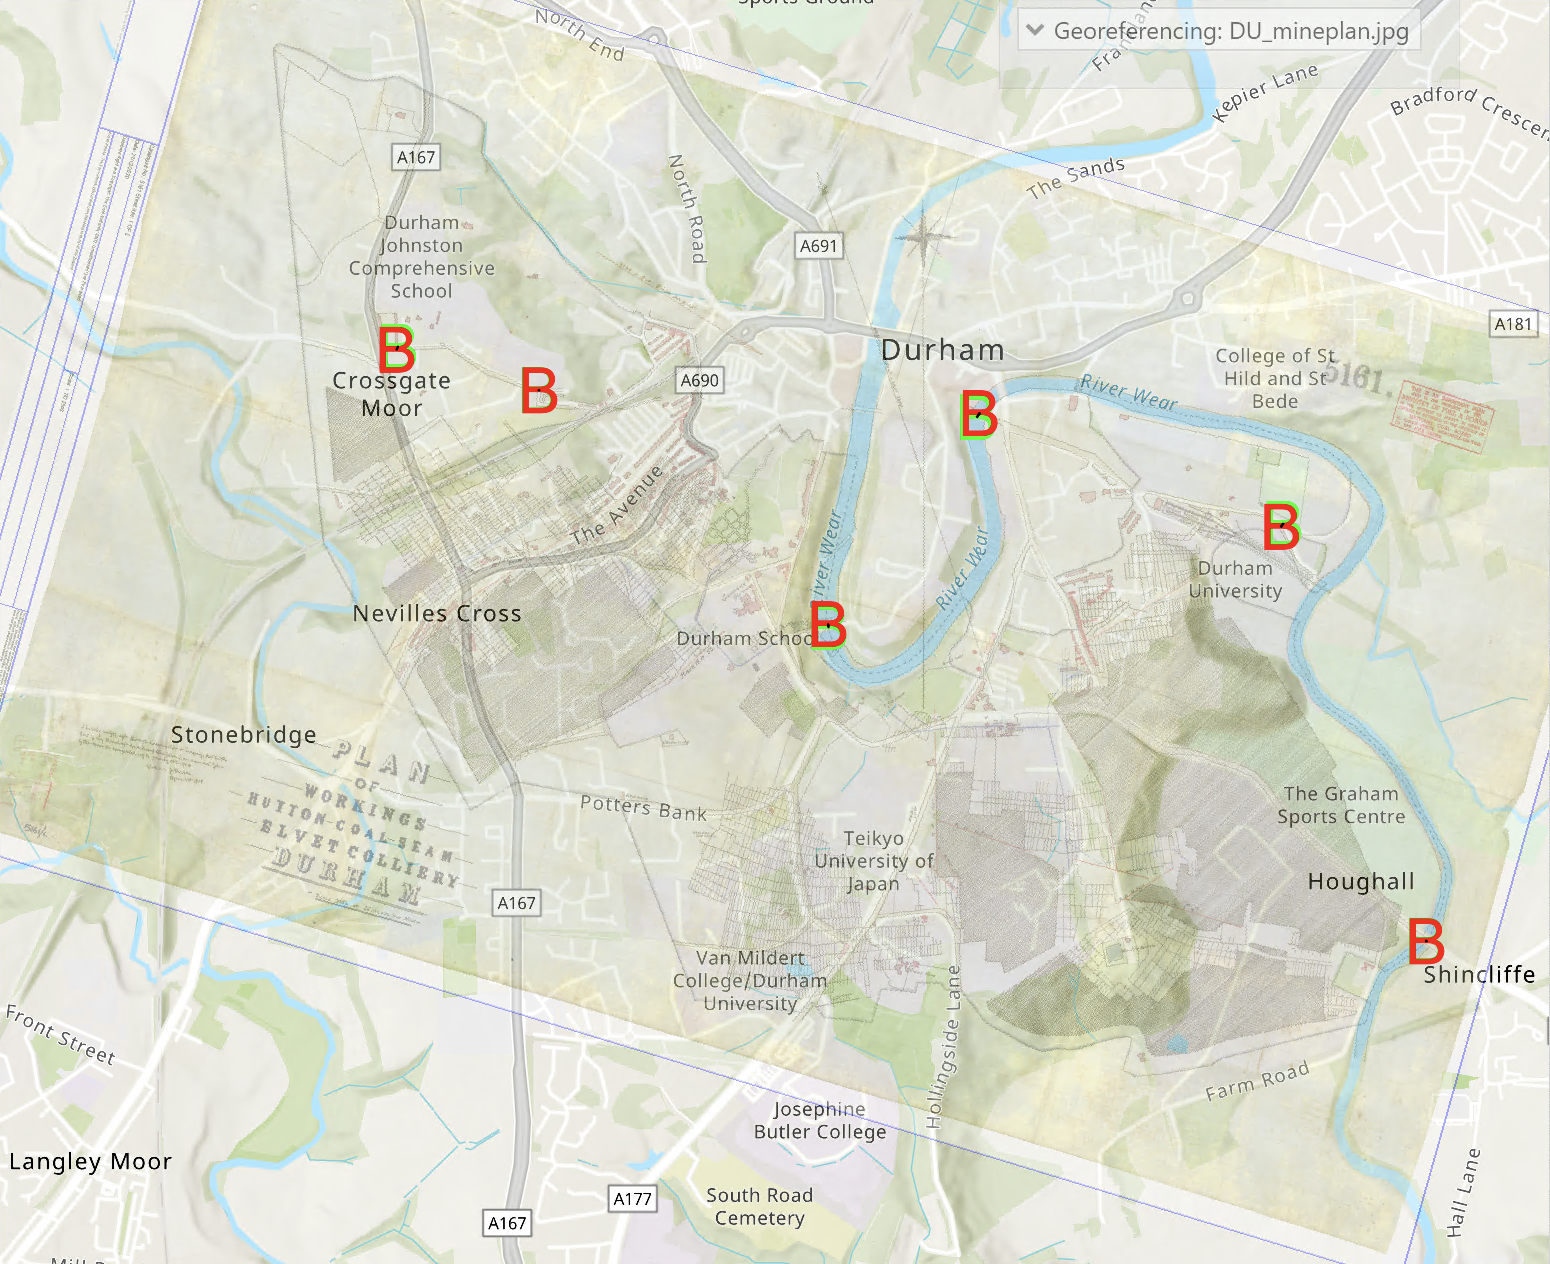
\includegraphics[scale=0.5]{figures/georeferencing.png}
          \caption{Example of a georeferenced mine plan. The connection points used for georeferencing are illustrated as 'B' on the map.}
          \label{fig:georeferencing}
       \end{figure}
       \item Once you are satisfied with the georeferencing, click 'Save' and then 'Close Georeference'.
    \end{enumerate}
\end{enumerate}
\subsection{Digitising roadways and galleries}
Now we can start with the digitisation. We'll start with adding the mine galleries and roadways ('pipes') in the room-and-pillar parts of the mine workings, and then we'll add any 'goaf' area for the long-wall mining parts of the mine workings later on. Digitising the galleries and roadways is done as follows. 

Note: Please strictly follow the following steps to digitise the mine workings, carefully check and draw the intersection points either between galleries or between galleries and goaf.
\begin{enumerate}
    \item In the Catalog pane, expand 'Databases' to see the pipes in its contents.
    \item Right-click on the {\tt .gdb} file inside the 'Databases', and choose New $\Rightarrow$ Feature Class. Choose a name (e.g. 'pipes'). In 'Feature Class Type', choose 'Line'. Un-tick the 'Z-values' option, since we will assume that seams are horizontal, and will add a uniform depth for the seam later. Click 'Next' multiple times to check all other options, but default values are probably fine. Click 'Finish' to initialize the dataset.  
    \item Click the output data set that was just created ('pipes'?) in the Contents pane.
    \item Click the Edit tab (if you run ArcGIS Pro via Appsanywhere, choose the Edit tab in ArcGIS Pro, not the one for the Parallels Client).
    \item Click 'Create' to start creating the pipes. A 'Create Features' pane will now appear as a second tab next to the 'Catalog' pane on the rhs. 
    \item Click on the 'pipes' item in the 'Create Features' pane. A blue box with different options will appear. Make sure the 'line' option 
\includegraphics[height=\baselineskip]{figures/line.png} is highlighted. 
    \item Expand the 'Snapping' item in the top ribbon to make sure the snapping tool is switched on. This will make sure that lines will be snapped together if the end point of a new line is close enough to a previous line. 
    %\item Now create a few lines. So click at starting point, and double-click at end point, without intermediate points. If a new starting/end point is close enough to a previously created line, text next to the cross on the map will appear, e.g. 'pipes: Edge'. This indicates that the point of the new line will snap onto the existing line, so that they become connected pipes. 
    \item Now create a few lines. It can help save time if you draw the lines in a certain order(for example, horizontal first and then vertical). So click at starting point, and click once at each crossroad to make a vertex and double click at end point. It will look like figure \ref{fig:long_lines}. When you finish drawing horizontal lines, you start to draw vertical lines as Figure \ref{fig:double_lines}. When you approach each crossroad point, some thing like "pipes: vertex" will appear, you can click on that vertix to guarantee two pipes intersect on that vertex.
    
    \begin{figure}[h]
        \centering
        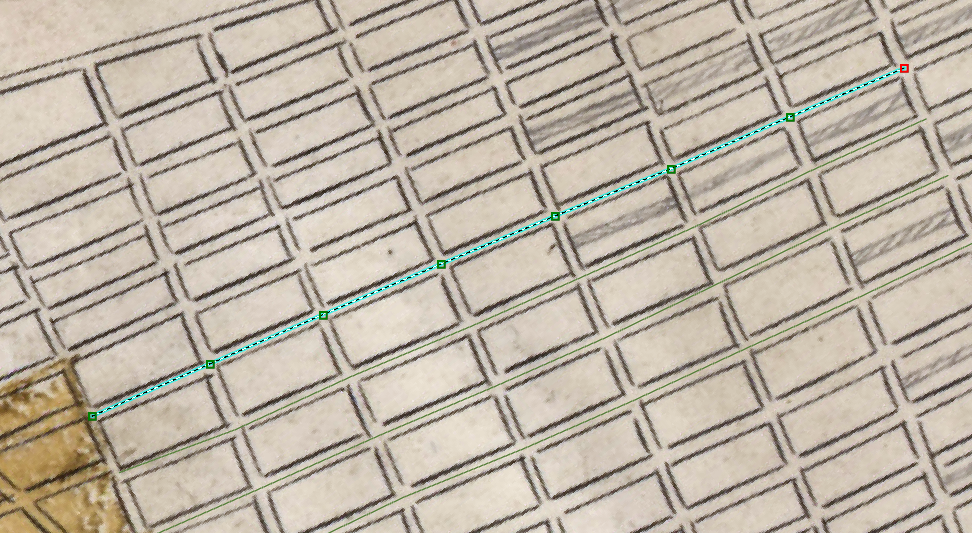
\includegraphics[scale=0.4]{figures/manual1.png}
        \caption{%The GEMSToolbox requires that each gallery is defined separately between crossroads. But in ArcGIS, we can create long lines that encapsulate multiple galleries (e.g. blue line in this figure). These will be separated into individual galleries later.
        Draw lines in a single direction}
        \label{fig:long_lines}
    \end{figure}

        \begin{figure}[h]
        \centering
        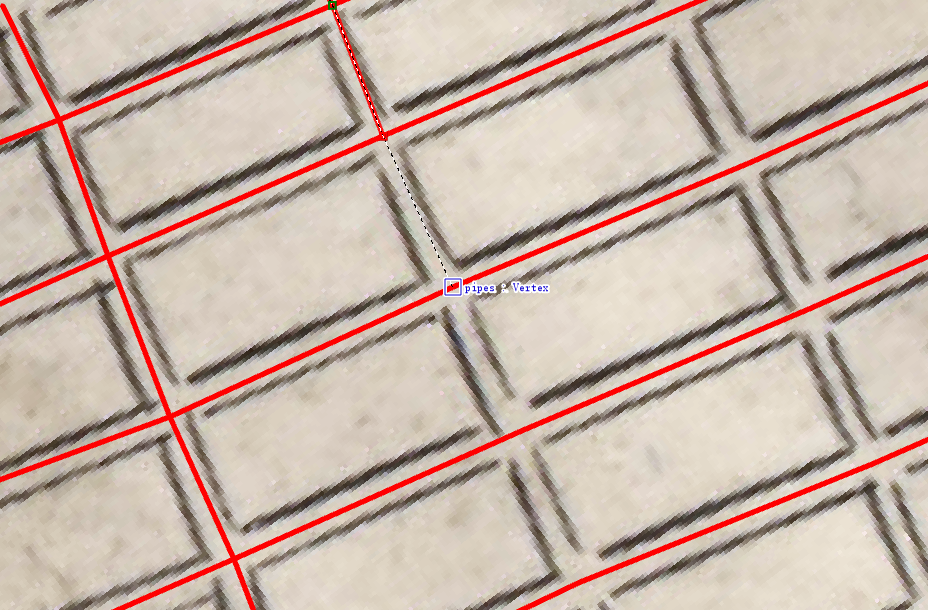
\includegraphics[scale=0.5]{figures/manual2.png}
        \caption{Draw lines in the other direction to intersect with the previous lines}
        \label{fig:double_lines}
    \end{figure}
    % As illustrated in Figure \ref{fig:long_lines}, you can create long lines that will cross multiple crossroads by just clicking the starting point and double-clicking the end point of that long line (i.e. don't click on the crossroads that the line crosses). Later on, we'll break up the long line into a series of shorter lines that run from one crossroads to the next, using a Python script. 
    \item to see previously created lines more clearly, right-click 'pipes' in the Contents pane, and choose 'Symbology', which creates a 'Symbology' tab in the rhs pane. Double click 'line' on the right side of the 'Symbol' in that Symbology pane, and then on 'Properties' next to 'Gallery'. Now change the thickness of the line to 3pt or 4pt, and choose a bright, clearly visible colour. Click on 'Create' again to continue creating more lines. 
    \item if you need to modify a line (e.g. because it doesn't snap into a neighbouring line', click on 'Modify', then click-and-drag the end point of the line you want to move to its new position.
    \item If you need to delete a previously created line, then in the 'Edit' tab, drop-down the 'Select' option, choose 'Line', then double-click the line you want to delete, and right-click and choose 'Delete' to remove 
    \item Once you are finished (or temporarily suspend adding more pipes, press 'Save'. To delete a 'goaf' area, follow the same procedure, but choose 'Polygon' instead of 'Line' in the 'Select' drop-down menu. 
\end{enumerate}
\subsection{Digitising goaf areas}
If the mine workings contain any goaf area, then these need to be digitised as well. If no goaf areas are present, or if you want to add those later, you can jump straight to the next section. 
Digitising the goaf areas is done with a similar procedure as for the galleries and roadways. 
\begin{enumerate}
    \item In the rhs pane, open the 'Catalog' tab again. 
    \item Click on triangle in front of 'Databases' to look at its contents.
    \item Right-click on the {\tt .gdb} file inside the 'Databases', and choose New $\Rightarrow$ Feature Class. Choose a name (e.g. 'goaf'). Un-tick the 'Z-values' option again. Click 'Next' multiple times to check all other options, but default values are probably fine. Click 'Finish' to initialize the dataset.  
    \item Click the output data set that was just created ('goaf'?) in the Contents pane.
    \item Click the Edit tab, and then 'Create' to start creating the goaf area. 
    \item In the 'Create Features' pane click on the 'goaf' item. 
    A blue box with different options will appear. Make sure the 'polygon' option 
\includegraphics[height=\baselineskip]{figures/polygon.png} is highlighted. 
    \item Make sure the snapping tool is again switched on. 
    \item Next, with a series of single-clicks, outline the corners of a goaf area and also click when meeting the endpoint of pipes to ensure connections between goaf and galleries(Figure \ref{fig:goaf_lines}). Double-click on the penultimate point (not on the point you started with, since ArcGIS will automatically close the polygon after the final point is added.
    \begin{figure}[h]
        \centering
        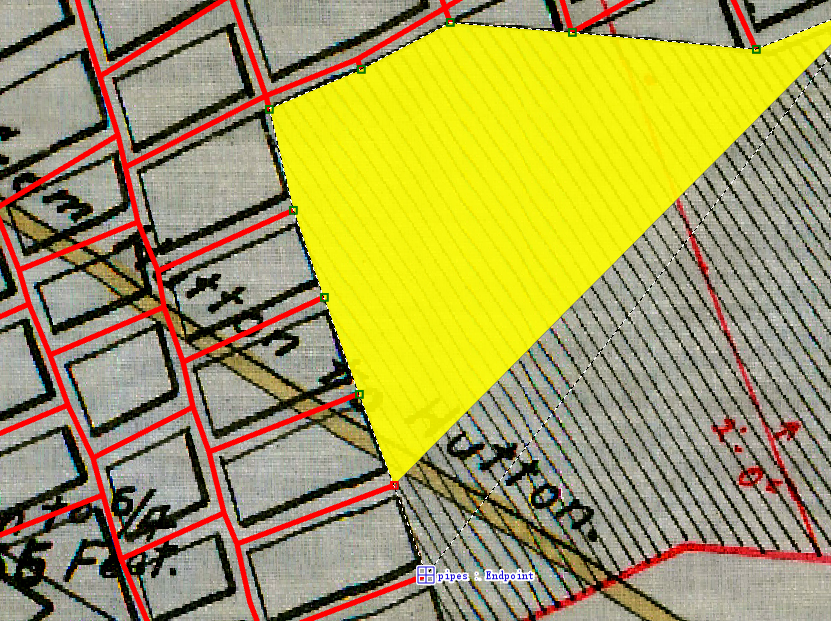
\includegraphics[scale=0.4]{figures/manual3.png}
        \caption{Draw goaf outlines to intersect with the endpoints of pipes}
        \label{fig:goaf_lines}
    \end{figure}
    
    %\item Note: Make sure that any connections between the goaf and the gallery features are done at \textit{vertices}. Connecting to edges of the goaf might cause issues unless snapping (explained below) is used.
    \item Repeat the last task for any other goaf areas you want to add. 
    \item Once finished, press Save again. 
\end{enumerate}
\subsection{Preparing data for the GEMSToolbox}
% Once you are happy with your pipe (and goaf) network, we need to do a few additional tasks, such as breaking up the long lines (see Figure \ref{fig:long_lines}) into individual galleries, and connecting pipe and goaf networks. These are all doneautomatically using a Python script that runs through ArcGIS. To run this, perform the following tasks: 
Next a Python script is loaded in ArcGIS to perform the digitization. The pipe nodes will be numbered.

\begin{enumerate}
   \item Download the latest version of the GEMSToolbox.
   \item Copy the file {\tt src/external\_functions/GEMSToolbox.py} to the ArcGIS project folder.
   \item Open the Python window in ArcGIS from the 'View' tab, by clicking 'Python Window', which will create an additional Python window at the bottom of the ArcGIS tool. 
   \item Open the GEMSToolbox.py file using a text editor (e.g. textedit), and copy the lines from "{\tt \# COPY FROM THIS LINE ...}" to "{\tt \# ... TO THIS LINE ...}" into the ArcGIS Python window. Press the "Enter" key once or twice to run the pasted commands. This will load in the GEMSToolbox set of Python commands into ArcGIS. Mac users, note that if you run ArcGIS via Appsanywhere, then you need to use the MS Windows shortkey for 'Paste' (i.e. Control-V, not Command-V). 
   \item Make sure the Map view is enabled in ArcGIS otherwise running the commands below will result in some errors.
   % \item OPTIONAL STEP: If you did not create any goaf areas, or if you do not wish to fine tune your goaf areas, you can skip this step. Note that this step will be automatically carried out by the script using a predefined set of parameters which will work if you have digitised your goaf areas accurately. Otherwise, you now need run the following command to 'snap' the goaf layer to the nearby galleries:
   %\begin{quote}
       %{\tt GEMSToolbox.snap\_porous\_zones\_to\_galleries(<goaf>,\\ <galleries>,<grid>,<radius>,<remove>)}
   %\end{quote}
   %(all on one line) in which: 
   % \begin{itemize}
       %\item {\tt <goaf>} the name of the Feature Class containing the goaf areas in double quotes (e.g. {\tt "goaf"}),
       %\item {\tt <galleries>} is the name of the Feature Class that contains the galleries/roadways within double quotes (e.g.: {\tt "pipes"}), 
       %\item {\tt <grid>} The algorithm will first create a dense grid of points every {\tt <grid>} meters around the polygon and will try to snap each of those points to a nearby gallery ({\tt 10} meters is a good value), 
       %\item {\tt <radius>} The algorithm will then search for {\tt <radius>} meters around each of those points for any nearby galleries to snap to. ({\tt 30} is a good value),
       %\item {\tt <remove>} The algorithm will finally remove obsolete grid points if closer together than {\tt <remove>} meters ({\tt 5} is a good value).
       %\item Note that this symbol {\tt <>} for each item should be removed after you replace them using specific values.
    %\end{itemize}
    %For example, the command could be as follows:
    %\begin{quote}
       %\texttt{GEMSToolbox.snap\_porous\_zones\_to\_galleries("goaf","pipes", 10, 30, 5)}.
       %\end{quote}
    
    %This will create a new Feature Class {\tt <goaf>\_snapped}, e.g. "{\tt goaf\_snapped}". 
   \item Next run the following Python command in the ArcGIS Python window: 
   \begin{quote}
       {\tt GEMSToolbox.generate\_shapefile(<gallery>, <depth>, <goaf>, 
       
       <snap\_porous\_zone>)}
   \end{quote}
   in which: 
    \begin{itemize}
       \item {\tt <gallery>} is the name of the Feature Class that contains the galleries/roadways inside double quotes (e.g.: {\tt "pipes"}), 
       \item {\tt <depth>} the depth of the coal seam in meters below the surface (e.g. {\tt -65}), 
       \item {\tt <goaf>} (optional argument) the name of the Feature Class containing the snapped goaf areas created in the previous step, inside double quotes (e.g. {\tt "goaf"}  or {\tt "goaf\_snapped"} if you used the optional step 5.) If you have no goaf areas, then leave out the last argument.
       \item {\tt <snap\_porous\_zones>} If you are confident that your goaf areas have been correctly connected to the galleries and then set to False. Therefore carefully check your connections before you take this step.

        % (optional argument)} set to True to enable the automatic goaf snapping feature (recommended if you have not manually snapped every single connected galleries to \textit{vertices} of your goaf areas).  %(or you have ran the optional step 5 above)and you do not want them altered 
       \item Note that this symbol {\tt <>} for each item should be removed after you replace them using specific values.
    \end{itemize}
    One example is like: \texttt{GEMSToolbox.generate\_shapefile("pipes", -65, "goaf", "False")}

    \item This Python script might take a while to run, particularly if your digitised mine system is large. Once finished, it produces a number of files with the same base name, as listed in the Python window (typically {\tt complete\_set\_feature\_1}. The first copy of the file is saved into your ArcGIS project database, the second is located into your project directory to be easily accessed. Copy all the {\tt complete\_set\_feature\_1} files located into the project directory over to the {\tt maps} folder of the GEMSToolbox (you may want to create a subfolder inside {\tt maps} to keep the folder tidy). This completes the digitisation process in ArcGIS Pro. 

    \item If you are confident all your connections between pipe lines and goaf polygons are perfectly done as the above steps without missing any connections between two nodes, you can run your model using GEMSToolbox smoothly.  However, you might meet problems sometimes, especially when you run the model with complex goaf zones. If such, you need to adjust the parameters Qth and flow\_error\_threshold. Their default values are set to 1E-7 and 1E-15, respectively. In most cases, you can gradually increase Qth in Excel sheet to a a bit larger value, but better not greater than 1E-4. If the problem still can't be solved, please contact yuxiao.wang2@durham.ac.uk.
    
\end{enumerate}

\section{Digitising mine plans with QGIS}
\subsection{Preparation}
To use and set up QGIS for the purpose of mine plan digitisation, the following tasks are needed:
\begin{enumerate}
    \item Install the latest stable version: for this, the user is referred to \href{https://docs.qgis.org/3.34/en/docs/user_manual}{the QGIS website}, Section 5.1.
    \item Start QGIS
    \item Basemaps: QGIS doesn’t start automatically with a basemap. The first time, you need to install basemaps: 
    \begin{enumerate}
        \item Install a plugin to enable that. Choose top menu "Plugins" $\rightarrow$ "Manage and Install plugins", and find "QuickMapServices" in list on the left. Install and enable the plugin
        \item Install the main list of standard maps: 
        Choose top menu "Web" $\rightarrow$ QuickMapServices $\rightarrow$ Settings. Click on tab "More Services", and choose "Get contributed pack".
        \item Once basemaps are installed, choose your basemap from top menu "Web" $\rightarrow$ QuickMapServices.
    \end{enumerate}
    \item Set the coordinate system to an orthogonal British National Grid system (or equivalent if working on areas outside the UK): at the bottom-right of the QGIS window, click on the CRS item ("Current CRS: ..."). In 'Filter', type "EPSG:27700", and choose "EPSG:27700 - OSGB36 / British National Grid", then click "OK". 
\end{enumerate}
\subsection{Georeferencing mine plans}
Now import the mine plan to be georeferenced:
\begin{enumerate}
    \item Top menu "Layer" $\rightarrow$ "Georeferencer". This opens a new window. 
    \item Choose the map file to be imported: top menu "File" $\rightarrow$ "Open Raster …". This opens the map in this Gereferencer window.
    \item Go to top menu "Settings" $\rightarrow$ "Transformation Settings". Set the “Transformation Type” to "Polynomial 1" (default is "Linear" which does not work, since it doesn’t rotate maps).
    \item Choose  the "Output file" where the georeferenced version of the file will be stored. 
    \item Tick the box "Use o for Transparency when needed": this will avoid a black ‘frame’ around the map if the map needs rotation once it is overlain onto the basemap. 
    \item Leave the other options as default and click "OK".
    \item Set at least 4 control points, which are points on the map and the corresponding point on the basemap:
    \begin{enumerate}
        \item Zoom in/out of the map in the georeferencer (without clicking!) to the location of the first control point
        \item Click on the map to define the first control point
        \item Now a new window "Enter Map Coordinates" appears: click on "From Map Canvas" in bottom-left to choose the corresponding point on the basemap, and this will redirect you to the basemap in the main QGIS window.
        \item Zoom in/out (again without clicking) to the corresponding point on the basemap and click at the location.
        - Now the "Enter Map Coordinates" window appears in front again. Click on “OK” in there. Now your first control point is created, and the “Georeferencer” window appears in front. 
        \item Repeat these steps for the 2nd and following control points. 
    \end{enumerate}
    \item Once you are happy with the control points, click on the green triangle button in the georeferencing window (or choose top menu "File" $\rightarrow$ "Start Georeferencing". Your georeferenced map will now appear on top of the basemap in the main QGIS window as a new layer. 
    \item Change the transparancy of the map by right-clicking on the map layer, choose "properties" (which opens the “Layer properties” window), choose "transparancy" in the list on the left. At the top, move the “Global Opacity” bar to around 50\%. Press "OK".
    \item Now you should be able to see both the map and the basemap underneath, and you can check if the map is properly georeferenced. 
    'item If you want to make changes, the "georeferencer" window should still be open, so you can remove control points (right-click on the point in the table, and choose remove), or add more points, then repeat the "Start Georeferencing" again, which will create another layer. Then remove the first map layer, since you only need the new one. 
\end{enumerate}
Don’t forget to regularly save the project: top menu "Project" $\rightarrow$ "Save".

\subsection{Digitising a mine plan}
Now that mine plan is imported and georeferenced, the next step is to digitise the mine plan. We first digitise any galleries and roadways, and then any goaf areas. If your mine plan only contains galleries/roadways or only contains goaf, then proceed with just digitising those only. Digitising x-y coordinates for any mine plan features is explained in Sections \ref{sec:digitising_galleries} and \ref{sec:digitising_goaf}. Section \ref{sec:digitising_depth} explains how to digitise the depth of a mine plan, either as a constant-depth flat plane, or as a variable-depth dipping or curving plane.

\subsubsection{Digitising galleries and roadways}
\label{sec:digitising_galleries}
To create a network of galleries: 
\begin{enumerate}
    \item Choose "Layer" $\rightarrow$ "Create Layer" $\rightarrow$ "New Shapefile Layer ...". Click on the 3 dots to choose a file name and appropriate path (just typing a file name in the box left of the 3 dots puts the file in the default (and probably wrong) folder). Choose: "Geometry Type" $=$ "LineString", "Coordinate system" = "EPSG:27700 -OSGB36 / British National Grid" (or equivalent if working dealing with an area outside the UK). Leave all other parameters blank or default, and click "OK"
    \item Now a new layer is created, visible in the QGIS "Layers" window, together with the map: click on the layer to highlight it. 
    \item Click on the pencil icon ("Toggle Editing") in the 2nd row, and then on the Line-with-Star icon ("Add Line Feature") to the right of it.
    \item Switch on the snapping tool: "Project" $\rightarrow$ "Snapping Options". A thin, wide window appears with all options: first box: snapping $=$ on (grey instead of white); third box: tick Vertex, Segment, Line Endpoints. Close the window.
    \item Now the mouse point should have a 'target’ shape, and you can start creating lines. Click on the start point, then on the end point of the line. Then right-click and click ‘OK’. Repeat this for next lines. Multi-segment lines should work as well.
    \item Note that long lines crossing other lines is fine: the postprocessing method will automatically split these long lines in individual segments. 
    \item When finished, click on the pencil icon again, and choose the option to save the changes.
\end{enumerate}

\subsubsection{Digitising goaf areas}
\label{sec:digitising_goaf}
To create one or more goaf areas: 
\begin{enumerate}
    \item Choose "Layer" $\rightarrow$ "Create Layer" $\rightarrow$ "New Shapefile Layer ...". Click on the 3 dots to a choose file name and appropriate path (just typing a file name in the box left of the 3 dots puts the file in the default (and probably wrong) folder). Choose: "Geometry Type" $=$ "Polygon", "Coordinate system" = "EPSG:27700 -OSGB36 / British National Grid" (or equivalent if working dealing with area outside UK). Leave all other parameters blank or default, and click "OK"
    \item Now a new layer is created, visible in the Layer window, together with the map: click on the layer to highlight it. 
    \item Click on the pencil icon ("Toggle Editing") in the 2nd row, and then on the Green-polygon-with-Star icon ("Add Polygon Feature") to the right of it.
    \item Make sure that the snapping tool is still on. Note that, for GEMSToolbox to create a viable solution, all galleries and goaf areas need to be connected, so your goaf area should have at least one point in common (i.e. snapped to) a node of the line galleries. Also note that galleries and goaf areas should not overlap. This means that any edge of the gaof zone cannot also be a gallery.
    \item Now the mouse point should again have a 'target’ shape, and you can start creating the outline of the first polygon. Click on the start point, then subsequent points. When you are 'back' near the start point, don't click on the start point again, as the polygon feature will automatically close the polygon. Now right-click and click ‘OK’. \item Repeat this for any subsequent polygons. 
    \item When finished, click on the pencil icon again, and choose the option to save the changes.
\end{enumerate}

\subsubsection{Digitising depth of mine plans}
\label{sec:digitising_depth}
If a mine plan is modelled using a fixed depth for the entire plan, this Section \ref{sec:digitising_depth} can be skipped, and this depth is dealt with in Section \ref{sec:QGIS2GEMS}. 

If a mine plan significantly deviates from being flat, then its depth needs to be explicitly digitised. For that, we need several points on the mine plan where depth is known. The geographical spread of these points should cover the extent of the digitised mine plan in Sections \ref{sec:digitising_galleries} and \ref{sec:digitising_goaf}. The following digitisation method will create a smooth 3-D layer as QGIS shapefile that interpolates between the depth points (but won't extrapolate beyond the lateral extent of those depth points). The x-y coordinates of the features digitised in Sections \ref{sec:digitising_galleries} and \ref{sec:digitising_goaf} will be 'draped' onto this 3-D layer to provide a z-coordinate for every x-y coordinate. 

The following QGIS procedure should be used: 
\begin{enumerate}
    \item Create a QGIS layer with depth points: 
    \begin{enumerate}
        \item Choose "Layer" $\rightarrow$ "Create Layer" $\rightarrow$ "New Shapefile Layer"
        \item Choose a file name for the 3-D layer (make sure to choose the correct folder!)
        \item Choose Geometry type = Point
        \item "New Field:"
        \begin{enumerate}
            \item "Name" = "Elevation" (suggested: any name is fine, in this manual "Elevation" is assumed further down)
            \item "Type" = "Decimal (double)"
            \item Click "Add to Fields List"
        \end{enumerate}
        \item Click "ID" in Fields List and then click on "Remove Field" below the list
        \item Click "OK"
    \end{enumerate}
    \item Highlight the new layer in the "Layers" panel
    \begin{enumerate}
        \item Click the 'pencil' icon ("Toggle Editing")
        \item Click the 'star-and-three-dots' icon ("Add Point Feature")
        \item Click at a point where depth is known; When asked for "Elevation", enter a depth value in meters and click "OK"
        \item Repeat this for all points you want to include for interpolation of the 3D depth layer.
    \end{enumerate}
    \item Open the "Processing Toolbox" if not already open ("Processing" $\rightarrow$ "Toolbox")
    \begin{enumerate}
        \item Type "IDW interpolation" in the Search box
        \item Choose "Interpolation $\rightarrow$ "IDW Interpolation". This will open a new window. N.B. this will use IDW $=$ Inverse-Distance-Weighting", which creates a smooth layer. If you prefer linear interpolation, there is another interpolation type called "TIN Interpolation". This option is not discussed here, but works very similar to IDW interpolation. 
        \item Choose "Vector Layer" $=$ your point layer that you've just created
        \item This should now show "Elevation" as attribute. Click the green "+" button
        \item Scroll down in the window to set "Extent" $=$ "Calculate from Layer", and choose your point layer. Other extent options might be worth trying if you are interested.
        \item Click "Run" and it should produce a new later with smooth depths between your set points. This file will be stored under the same name with a .tif extention, indicating that is a 'geotiff' file type. This file name will be needed in the next section. You may want to move this new layer to below your other layers so that it is plotted 'behind' those other layers. 
    \end{enumerate}
\end{enumerate}

\subsection{Convert line and polygon features into GEMSToolbox shapefiles}
\label{sec:QGIS2GEMS}
Now some processing of those line and goaf features is needed to make them suitable for the GEMSToolbox calculation: multi-segment lines need to be split into individual lines, crossing lines need splitting up, lines and polygon features need to be merged, nodes need a unique numbering, and those nodes need attributes to store additional information (such as which line of polygon each node belongs to). This can all be done automatically using a Python script that can run inside QGIS. Here are the steps to enable this: 
\begin{enumerate}
    \item Copy the script ${\tt QGIS2GEMSTb.py}$ from the GEMSToolbox folder ${\tt src/external\_functions}$ to the QGIS project folder.
    \item Open the {\tt QGIS2GEMSTb.py} file using any text editor. Scroll to the main code at the end of the file, and modify the following two lines: 
    \begin{verbatim}
       line_file   = "pipes.shp"
       goaf_file   = "goaf.shp"
    \end{verbatim}
    by inserting the name you created for the shapefiles for the galleries and goaf features. 
    If you only have digitised roadways, just leave the ${\tt goaf\_file}$ empty:
    \begin{verbatim}
       goaf_file   = ""
    \end{verbatim}
    or provide a non-existent filename: if the script cannot find a file, it will assume no digitised goaf area is present. Similarly, if you only have digitised one or more goaf zones, provide an empty or non-existent ${\tt line\_file}$ :
    \begin{verbatim}
       line_file   = ""
    \end{verbatim}
    By default, the output of the script will be written to a shapefile defined in the line: 
    \begin{verbatim}
       GEMSTb_file = "QGIS_digitised_map.shp"
    \end{verbatim}
    This can be modified if needed/desired, e.g. when dealing with multiple worked seams (see below).
    
    If you want a fixed depth of your mine plan, set the parameter to the right value, e.g. 100 m depth:
    \begin{verbatim}
       height = -100.
    \end{verbatim}
    Note that a negative value of ${\tt height}$ represents the depth of the mine workings. If you have created a variable depth layer in Section \ref{sec:digitising_depth}, enter that for the variable ${\tt z\_layer\_file}$, e.g.:
    \begin{verbatim}
       z_layer_file = "slope_raster_IDW.tif"
    \end{verbatim}
    As for the other file names, if the file name is empty or the file does not exist, then the script will assume that no variable depth is required, and the value of the parameter ${\tt height}$ will be used instead.
    
    Save the changes when ready.
    \item In QGIS, Open the Python Console in "Plugins" $\rightarrow$ "Python console". This should open the console below your map.
    \item Inside the console, click the "Show Editor" icon (lined paper-with-pencil icon). 
    \item Inside the newly opened editor, click the "Open Script ..." icon (folder icon) to open the ${\tt QGIS2GEMSTb.py}$ script.
    \item Run the script by pressing the "Run" button (green triangle).
    \item If all went well, it should produce some output ending with "STEP 6: Adding GEMSTb attributes COMPLETED". It will have created a set of files starting with \verb|QGIS_digitised_map.*|. 
    \item In the GEMSToolbox folder system, go to the folder ${\tt data/maps}$ and create a new folder for the digitised mine plans. Copy all the \verb|QGIS_digitised_map.*| files from the QGIS project folder to this new folder.
\end{enumerate}
The process of creating lines and polygons can be repeated if multiple mine workings are modelled together. Each worked seam then gets its own GEMSToolbox shapefile. But keep in mind that, if you create those different mine workings in the same QGIS folder, the files \verb|QGIS_digitised_map.*| will need different names for the different seams. 

\vspace{0.5cm}
\noindent\fbox{
    \parbox{\textwidth}{
        Warning: the QGIS2GEMSTb.py script is a relatively recent addition to the GEMSToolbox, and the present beta version may need some further implementations. If anything does not work properly, or you would like to request additional features or functionalities, please contact Jeroen van Hunen at \verb|jeroen.van-hunen@durham.ac.uk|.
        }
    }
\vspace{0.5cm}

\section{Running GEMSToolbox with the newly created digitised map}
\subsection{Creating a custom input file}
\begin{enumerate}
    \item Using the MacOS Finder or Windows Explorer navigate to {\tt <homeGEMSTb>/data} then make a copy of the {\tt Grid\_demo.xlsx} or any of the templates provided.
    \item Rename the copy to anything you want, but keep the Excel {\tt .xlsx} extension. For now we will call this {\tt CustomScenario.xlsx}
    \item Open your {\tt CustomScenario} file in a spreadsheet editor. You can now customise any of the parameters as you wish using the information provided in the keyword glossary (Section \ref{sec:glossary}) below. Note that if a parameter is not listed in the input file, the code will use its default value, as listed in Section \ref{sec:glossary}.
   \item On the command line, move to the {\tt <homeGEMSTb>} folder, and run the following command to start the calculation: \\
   {\tt python GEMSTb.py data/CustomScenario.xlsx}
   \item If your input file contains multiple models (i.e. multiple columns), you can run the code in parallel: \\
   {\tt python GEMSTb.py data/CustomScenario.xlsx --num\_workers N}\\ where {\tt N} is the numbers of parallel threads you would like to use.
\end{enumerate}

\section{View outputs}
\label{sec:view outputs}
The outputs of each Scenario input file are saved in the \texttt{outputs/[scenario\_filename]} folder.  
The outputs consist of:
\begin{itemize}
\item A {\tt .vtk} file for each of the runs in that scenario named: \texttt{[scenario\_filename]\_[tag]\_[runindex]}
\item A {\tt .csv} file which records the relative temperature of each outflow node in each run. The relative temperature $T_r$ is given by $T_r = T_{out}/\Delta T$, where $\Delta T = |T_{r,max} - T_{w,min}|$, i.e. the difference between maximum rock temperature and minimum water temperature. 
\end{itemize}
The {\tt .vtk} file contains all the output information as set in the input file, and these can be viewed using Paraview. Here are a few basic steps to create a plot to view the results. 
\begin{enumerate}
\item Open Paraview
\item Click on the folder icon 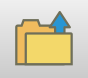
\includegraphics[height=\baselineskip]{figures/folder_icon.png} in the top-left corner, and navigate to the {\tt .vtk} file, press 'OK'.
\item click 'Apply'. You should now be able to view the temperature solution.
\item To view a different parameter (e.g. water velocity or hydraulic head), choose a different parameter from the drop-down menu on the second row that now states "T(C)".
\item To re-scale the colour bar to the full range of values, use the 
\includegraphics[height=\baselineskip]{figures/double-arrow_icon.png} icon.
\item To change the line width of the galleries, click to highlight the {\.vtk} file in the "Pipeline Browser" panel at the top-left, and then, in the "Properties" panel at the bottom-left scroll down to "Line Width".
\item To get information about a specific node in the network, click the 
\includegraphics[height=\baselineskip]{figures/dot?_icon.png} icon, and click 'OK'. Now zoom in onto the area of interest, and hover the mouse over a node to see the available information.
\item There are a lot of options to customise the plot further. One handy option in Paraview is that you can save the customised view as a 'state', and then load it back in later on, for the same or for a different data set. To do that, choose 'File' $\Rightarrow$ 'Save State...', which saves the state as a {\tt .pvsm} file. Next time you use Paraview, you can use the same state by, instead of using the 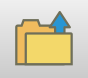
\includegraphics[height=\baselineskip]{figures/folder_icon.png} icon to load a {\tt .vtk} file, use 'File' $\Rightarrow$ 'Load State...', and choose the previously saved {\tt .pvsm} file. In the 'Load State Data File' option, choose 'Choose File Names', and choose the {\tt .vtk} file to display, then press 'OK'. The {\tt outputs} folder in the GEMSToolbox code already contains a {\tt .pvsm} file to get started. 
\item Change the background colour, find the 'Background' section in 'Properties', untick 'Use Color Palette For Background', click background button to choose suitable colour (Figure \ref{fig:background}).
 \begin{figure}[h]
        \centering
        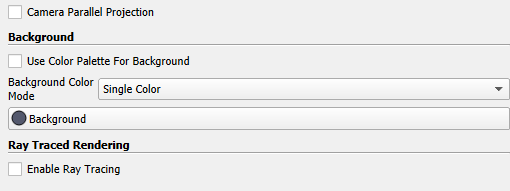
\includegraphics[scale=0.7]{figures/backgroundcolor.png}
        \caption{Change the background colour}
        \label{fig:background}
    \end{figure}
\item Change title/text font colour. When the background colour is changed, the legend title/text font colour might also need to be changed. Click 'edit colour map' 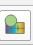
\includegraphics[height=\baselineskip]{figures/color icon.png} to open colour map editor. Then click 'Edit colour legend properties' button 
\includegraphics[height=\baselineskip]{figures/legend colour.png} to open 'Edit Colour Legend Properties', choose the suitable colour for legend title and text.


\end{enumerate}


\section{Input Keyword Glossary}
\label{sec:glossary}
This section describes the properties that can be set in the input file. Any property not set up in the input file will be read from the \verb|config/default_params.yml| file. The format of the parameters in the Excel input file is such that only numbers, strings, space, commas (,), and square brackets ([ ]) are allowed in the input Excel file.
2D arrays can be inputted as [1 2] [3 4] or [[1,2], [3,4]]. Formatting using other symbols like [1 2 ; 3 4] or 1 2 ; 3 4 is not allowed.

\begin{itemize}
\item {\bf a} (0.5): the damping oscillation factor applied to the flow at iteration n-1.
\item {\bf ArcGIS\_file\_name} (no default): the path to the shapefiles to be used to generate the geometry with \texttt{step\_load\_GIS\_geometry}. The format is 
        \texttt{[<directoryPath>/<fileName1>.shp, <directoryPath>/<fileNameN>.shp]}.
\item {\bf b} (0.5): the damping oscillation factor applied to the flow at iteration n.
\item {\bf connections} ([ ]): list of node ID doublets to create connecting pipes (e.g. to connect different seams)
\item {\bf Cp\_f} (4186 J/K/kg) specific heat capacity of the mine water 
\item {\bf Cp\_r} (960 J/K/kg) specific heat capacity of the rocks 
\item {\bf d\_set} (2.25 m) diameter of the mine galleries 
\item {\bf eps} (0.1 m): mine gallery roughness parameter 
\item {\bf fixed\_head\_node} ([[2, 0.0]]): node nr where hydraulic head is fixed 
\item {\bf flow\_error\_threshold} ($1.0 \times 10^{-15}$): numerical accuracy of the flow solver 
\item {\bf gis\_overrides} ( ):  parameters to be overriden using the value found in the GIS files.
\item {\bf grid\_height} (3): nr of grid points in y-direction (used for structured grids only) 
\item {\bf grid\_width} (3): nr of grid points in x-direction (used for structured grids only) 
\item {\bf gw\_darcy\_velocity} (0 m/s): Darcy velocity of the regional groundwater into the mine.   
\item {\bf h\_pipe\_length} (50 m): x-length of each gallery segment (used for structured grids only) 
\item {\bf Hydraulic\_conductivity} (0.03 m/s): Hydraulic conductivity of porous zones (goaf and collapsed/backfilled galleries) 
\item {\bf igeom} (\verb|step load_GIS_geometry|): specifies the geometrical function file to be used by the code. Two options are available: 1) \verb|step load_GIS_geometry| (will read structure from GIS shapefile), and 2) \verb|step_grid_geometry| (will generate uniform grid ) 
\item {\bf int\_d} (1000): nr points to evaluate the thermal interference between galleries 
\item {\bf k\_f} (0.58 W/m,K): fluid thermal conductivity 
\item {\bf k\_r} (2.6 W/m,K): rock thermal conductivity 
\item {\bf mat\_d\_prop} ([5.0] m: array to set different diameter to specific pipes specified with \verb|mat pipe_ids|
\item {\bf mat\_K\_prop} ([0.03] m/s: array to set different hydraulic conductivities to specific pipes specified with \verb|mat pipe_ids|
\item {\bf mat\_pipe\_ids} ([ ]): array to pipe IDs for which non-default diameter or hydraulic conductivity values apply. See also parameters mat\_d\_prop and mat\_K\_prop.
\item {\bf mat\_prop\_case} (1): the switch case code used to apply the material properties to the model (currently porosity and hydraulic conductivity). 1: sets porosity to 1 for all pipes (i.e. all pipes are considered open). 2: sets all the pipes to the porosity and hydraulic conductivity specified in the \textbf{porosity} and \textbf{Hydraulic\_conductivity} input keywords respectively. 3: uses a Perlin Noise map to set the porosity values of the pipes, and beyond a certain threshold (specified in \textbf{open\_th} keyword) all the pipes are considered open with a porosity of 1. The value specified in the \textbf{Hydraulic\_conductivity} input keyword is used as the hydraulic conductivity in all pipes. 4: like 3, but around a radius specified by the \textbf{well\_exclusion\_th} input keyword, where all pipes are considered open. 5: like 4 but instead of forcing open pipes around the wells, we force porous pipes. 
\item {\bf max\_sim\_time} (20 yrs): the maximum time it should take for water to reach the end of any given pipe. Beyond which the outflow temperature of a pipe will be considered to be that of the initial rock temperature.  
\item {\bf mesh\_density} (100 m): The maximum mesh size the model will try to achieve in 2D porous goaf areas. 
\item {\bf n\_steps} (10): the number of steps it takes the water to flow through a pipe.
\item {\bf no\_seams} (1): number of seams for scenario of regular structured grids (if igeom $==$ step load\_GIS\_geometry)
\item {\bf node\_outputs} (Tn T(C), head Head(m), tt\_n transit\_times(yrs), wells Well\_positions,
    n\_tree\_idx, Tree\_pos, node\_id node\_id]): specifies the desired nodal outputs to be saved in the vtk file for each run.  
        List of valid node outputs:
        \begin{itemize}  
            \item node\_id: the id of the node found in the underlying GIS files or/and ID to be used to set inflow, outflow, or fixed head nodes.
            \item Tn: the nodal temperatures of the model. 
            \item head: the nodal hydraulic heads of the model.
            \item tt\_n: the time it takes water to flow from the closest net inflow point to this node.
            \item wells: indicates the inflow (1), outflow (-1) and fixed head (0) nodes. All other nodes have a NaN value.
            \item n\_tree: the position of nodes in the tree used to sequentially solve the heat transfer.
        \end{itemize}
\item {\bf nu\_f} (1.2e-06 Pa s): dynamic viscosity of the mine water.
\item {\bf nyrs} (3 yrs): the number of simulation years is to be run for. 
\item {\bf open\_th} (0.5): threshold value of (random) porosity above which a pipe is considered 'open'. Applies to the cases where mat\_prop\_case $>$ 1.
\item {\bf pipe\_outputs} ([pipe\_id pipe\_id, vs Water\_velocity(m/s), Q\_real Flow\_rate(m3/s), poro\_e Porosity($\mathrm{m^3/m^3}$), Re Re(-), d Pipe\_diameters(m), alphas Alpha, rp R\_0, dT\_model Heat\_Model\_dT(C)]): specifies the desired pipe outputs to be saved as cell values in the vtk file for each run.
        List of valid pipe outputs:
        \begin{itemize}
            \item pipe\_id: the id of the pipes as held within the GEMS toolbox. 
            \item Re: the Reynolds number.
            \item v: the water velocity inside the pipe (m/s) assumed uniform. 
            \item Qv: the vectorised flow rate through the pipes (m$^3$/s). Saved as a vector in VTK with an x, y and z component.
            \item Q: the absolute flow rate through the pipes. Is equal to the magnitude of Qv.
            \item poro: the porosity of each pipe.  
            \item rp: the radial distance of the thermal front inside an infinite homogeneous porous rock.
            \item Tp: a vectorised value holding two components labelled x and y. x corresponding to the inflow temperature of the pipe and y to its outflow temperature.
            \item pmod: indicates which case of the statement is used in the heat calculation code. 
            \item Qdiff: the flow difference in the pipe between the last and penultimate iteration in the flow computation.
            \item K: hydraulic conductivity.
            \item d: pipe diameter.
        \end{itemize}
\item {\bf Porosity} (0.3): the porosity of the any backfilled or collapsed pipes.
\item {\bf q\_in} ([1]): array of injection node ID(s).
\item {\bf q\_out} ([3]): array of abstraction node ID(s).
\item {\bf qset} ([0.01] $\mathrm{m^3/s}$): the flow rate in/out of each injection and abstraction wells
\item {\bf Qth\_tree} (1.0e-07): the cut-off value for the flow comparison check used when disregarding a node for the computation of the flow tree required for the sequential heat calculations. This might need adjusting if porous pipes sections of the models are not added to the tree.
\item {\bf rho\_f} (1000 $\mathrm{kg/m^3}$): density of the mine water.
\item {\bf rho\_r} (2400 $\mathrm{kg/m^3}$): density of the rock mass surrounding the mine.
\item {\bf rng\_seed} (1): random number generatore seed used for random porosity models (when mat\_prop\_case $>$ 1)
\item {\bf seam\_spacing} (100 m): spacing of seams in regular grid models (when igeom $==$ step\_grid\_geometry)
\item \textbf{Tag} ( ): allows you to specify a tag that will be added to the output .vtk filename.
\item {\bf Tf\_ini} ([3] $\mathrm{{}^o}C$): array of the same length as for parameter q\_in with water injection temperature(s).
\item {\bf Tr} ([-0.032, 8.8] $\mathrm{{}^o}C/m$, $\mathrm{{}^o}C$): Rock temperature definition: first parameter is the vertical gradient, while the 2nd value is the rock temperature at the surface. 
\item {\bf v\_pipe\_length} (50 m): y-length of each gallery segment (used for structured grids only) 
\item {\bf well\_exclusion\_th} (30 m): avoid porous zones within well\_exclusion\_th from the injection or abstraction wells. 
\end{itemize}

\section{Adding additional parameters}
To compute some of your inputs you might want to perform intermediate calculations based on some additional parameters. To do this you can simply add another parameter, give it a name in the first column, with no spaces, and populate ALL the columns where a scenario is already defined. You can then use this parameter with Excel's inbuilt capabilities to compute your desired parameters. This should enable you to keep track of all the parameters used to obtain your inputs in the same file. Note that, 'loose' numbers in other parts of the spreadsheet will cause errors.

\section{Troubleshooting}
\subsection{ArcGIS common problems}
\subsection{GEMSToolbox common problems and errors}
\begin{itemize}
      \item \textbf{Gmsh configuration:} GEMSToolbox makes use of a meshing software Gmsh by calling Gmsh Python API. However, incorrect Gmsh configurations can occasionally result in errors. To ensure proper functionality, install Gmsh using the pip package manager command ``{\tt \bf pip install gmsh}'' rather than the Conda command {\tt conda install gmsh}. If the problem persists, you can download the standalone Gmsh executable directly from the official website: \url{https://gmsh.info/#Download}. Then run ``{\tt python GEMSTb.py <model>.xlsx <gmsh-path>}'', where {\tt <gmsh-path>}  refers to the path of the Gmsh executable. For example on Windows: {\tt \bf python GEMSTb.py .\textbackslash data\textbackslash testmineplan.xlsx D:\textbackslash gmsh-4.13.1-Windows64\textbackslash gmsh}. GEMSToolbox will call the external Gmsh excutable.
      \item GEMSToolbox versions from May 2025 or older were using an input file with a different format (using a horizontal rather than vertical layout). If you have 'old' input files that you would like to run with the latest version of GEMSToolbox, you can convert the input file to the new format using the Python script {\tt convert\_input\_xlsx.py}.
      To run the script: \\
      {\tt python convert\_input\_xlsx.py <old\_scenario\_file>}\\
      This will create a new input file in the folder where this script is run with {\tt \_transposed} in its file name. If needed, you can then rename this new parameter file and/or move it to the desired folder.
\end{itemize}

\subsection{Paraview common problems}
\begin{itemize}
      \item \textbf{Line width of cell attributes:} On MacOS systems, lines don't render correctly if the Line Width is larger than $1.0$. The problem is discussed in \href{https://discourse.paraview.org/t/cell-values-partly-disappear-when-editing-width-on-mac/11666}{this forum post}. A partial work-around is to convert the lines (i.e. cell data) into interpolated points (i.e. point data). To do this, click on the data set in the Pipeline Browser' which contains the line data. Then choose the 'Filters' tab, then 'Alphabetically', and then 'Cell Data to Point Data'. Choose your line data to plot, and you should be able to use larger Line Widths now. The difference is that the original line data has uniform line values, whereas the derived 'Cell Data to Point Data' dataset interpolates between the points on either end of the line. So for rapidly changing values, it might not be what you want. 
\end{itemize}
\end{document}
